\chapter{ METHODOLOGY}

\noindent
In this chapter, we present the methodological framework adopted for our study. We detail the processes of data preparation, question-answer generation, model training, and evaluation, as well as the development of the visualization tool. Each section outlines the specific steps and techniques employed to ensure the reliability and reproducibility of our results.

\section{Dataset preparation}

\noindent
This section describes the procedures followed to curate and preprocess the datasets used in our research. We explain the selection of data sources, the integration of supplementary geographic and road network information, and the steps taken to ensure data quality and consistency prior to analysis.

\subsection{Data sources}

We leveraged the comprehensive China crime dataset published by \cite{Zhang2025CrimeDatasetChina}. To provide geographic context, we integrated administrative boundary data for China \citep{GeoJSON2025China} and road network data from OpenStreetMap \citep{Vargas2021OSM}. This enabled proximity calculations between criminal incidents and nearby roads, a significant variable within our analytical framework. Full dataset columns details are provided in Appendix \ref{appendix:dataset}.

\subsection{Data sources cleaning and normalization}

The dataset underwent thorough cleaning procedures, including handling of missing values, consolidating category columns through LLM-based classification, and standardization of date formats. All text fields were subsequently translated to English. To maintain analytical focus, we concentrated on the three provinces exhibiting the highest crime incidence during the 2017-2019 period: \textit{Jiangsu}, \textit{Guangdong}, and \textit{Zhejiang}.

\subsection{Question-Answer generation}

To develop our question-answer dataset, we first created 100 question templates (inspired by \citep{Dai2024QASTKG, Contractor2020QATourism}), covering different types of inquiries including spatio-temporal, comparative, and causal questions about crime data. These templates were designed to be adaptable for crime datasets from other countries as well.

We expanded this initial set through question augmentation techniques used by \cite{Yin2024MuMathCode, Li2024MuggleMath, Jain2024MetaFineTuning}, specifically rephrasing (with temperature setting of 0.5) and alteration (with temperature setting of 0.75) via few-shot prompting (see Table~\ref{tab:question_type_counts}). These question categories are summarized in Table~\ref{tab:question_types}. Then, for each original question type, we selected random examples and developed Python code solutions manually. These hand-crafted solutions provided context for generating additional synthetic code answers using the DeepSeek V3 model with prompting (Appendix~\ref{appendix:prompts}) and nucleus-sampling \citep{Holtzman2020NucleusSampling, Ahmad2025OCRNVidia, Nvidia2024KaggleMath} (top\_p set to 0.95), generating new reasoning paths and coding approaches.


\begin{table}[H]
\centering
\begin{tabular}{lr}
\hline
\textbf{question\_type} & \textbf{\# count} \\
\hline
altered     & 3860 \\
paraphrased & 1732 \\
\hline
\end{tabular}
\caption{Distribution of question types in the dataset.}
\label{tab:question_type_counts}
\end{table}

\begin{table}[H]
\centering
\caption{Question types in the ChinaCrimeQACode dataset}
\label{tab:question_types}
\begin{tabular}{ll}
\toprule
\textbf{Question Type} & \textbf{Description} \\
\midrule
\texttt{spatial\_lookup} & Location-only questions \\
\texttt{temporal\_lookup} & Time-centric questions \\
\texttt{spatio\_temporal\_lookup} & Joint space-time filters \\
\texttt{comparative\_trends} & Rankings and evolution analysis \\
\texttt{causal\_contextual} & Event patterns and conditional queries \\
\texttt{hypotheticals\_counterfactuals} & Projections and counterfactual reasoning \\
\texttt{multi\_step\_aggregation} & Multi-step reasoning and aggregation \\
\bottomrule
\end{tabular}
\end{table}


\subsection{Dataset filtering}

To ensure quality, we verified that all LLM-generated Python solutions executed correctly. When errors occurred, we resubmitted queries to the LLM until either receiving a working solution or reaching the maximum retry limit. After that, we dropped the questions with no valid code solutions (limit exceeded, code with errors, or no code generated). Finally, we conducted manual reviews of all question-answer pairs to guarantee their quality.

\subsection{Dataset splitting}

The resulting dataset, which we named "ChinaCrimeQACode", contains around 5,000 question-code solution pairs, representing an adequate sample volume for effective model training \citep{Unsloth2024Dataset1}. We divided the dataset into training and test subsets using an 80/20 split (Table~\ref{tab:dataset_split}) to facilitate robust model training and comprehensive evaluation. The dataset is publicly available on HuggingFace for further research and development.
% This review process involved verifying that the answers were accurate, relevant, and aligned with the corresponding questions. We also ensured that the answers were concise and clear, making them suitable for use in our visualization tool.

\begin{table}[H]
\centering
\begin{tabular}{lr}
\hline
\textbf{Split} & \textbf{Count} \\
\hline
train & 4513 \\
test  & 1079 \\
\hline
\end{tabular}
\caption{Dataset split distribution.}
\label{tab:dataset_split}
\end{table}


% TODO: poner ejemplo de question-answer pair

\section{Prompt Structuration}
Prompts were carefully designed to ensure the model understood the task requirements and could generate accurate code solutions.  
We generate code solutions using a structured prompt (Figure~\ref{fig:prompt_structure}) that includes the following components:  
(1) a system message that sets the context for the model,  
(2) a dataset context where we provide each table description, including column names and types,  
(3) a question that specifies the task to be performed,  
(4) a critical-requirements section that outlines the specific constraints for code generation,  
(5) an output-format section that prescribes the expected response structure, and  
(6) an execution directive that instantiates the model to write the code solution.

\medskip
\noindent
\textbf{Prompt design in detail.}  
Figure~\ref{fig:prompt_structure} illustrates the layered architecture that guides the large-language model from high-level context to low-level implementation:

\begin{enumerate}
  \item \textbf{System Instruction:} Defines the agent’s role as an expert in geospatial crime analytics and explicitly enumerates the \emph{only} permitted libraries.  
  This early scoping mitigates hallucinations and enforces deterministic, reproducible outputs.
  
  \item \textbf{Dataset Context:} Supplies declarative metadata for the three interconnected GeoDataFrames: \texttt{crimes\_df}, \texttt{streets\_df}, and \texttt{geometries\_df}.  
  Column names, data types, and schema relations (e.g., point‐to‐line containment) are provided to prime schema awareness.
  
  \item \textbf{User Question:} A natural-language query that specifies the required spatio-temporal analysis.
  
  \item \textbf{Critical Requirements:} Lists fine-grained constraints the generated code must satisfy, including the function signature, CRS alignment checks, sanctioned libraries, and robust error handling.
  
  \item \textbf{Output Format:} Mandates that the response consist solely of a single \texttt{python} code block, disallowing any explanatory prose.  
  This rigidity greatly simplifies downstream execution pipelines.
  
  \item \textbf{Execution Directive:} Issues an imperative \enquote{BEGIN CODING IMMEDIATELY} that forces the model to produce executable Python as its very first token, eliminating meta-commentary.
\end{enumerate}

These six layers funnel the model from overarching context to executable detail, effectively functioning as a self-contained software specification.  
The complete version of the prompt is described in Appendix~\ref{appendix:prompts} for full transparency and reproducibility.

\begin{figure}[hbtp]
  \centering
  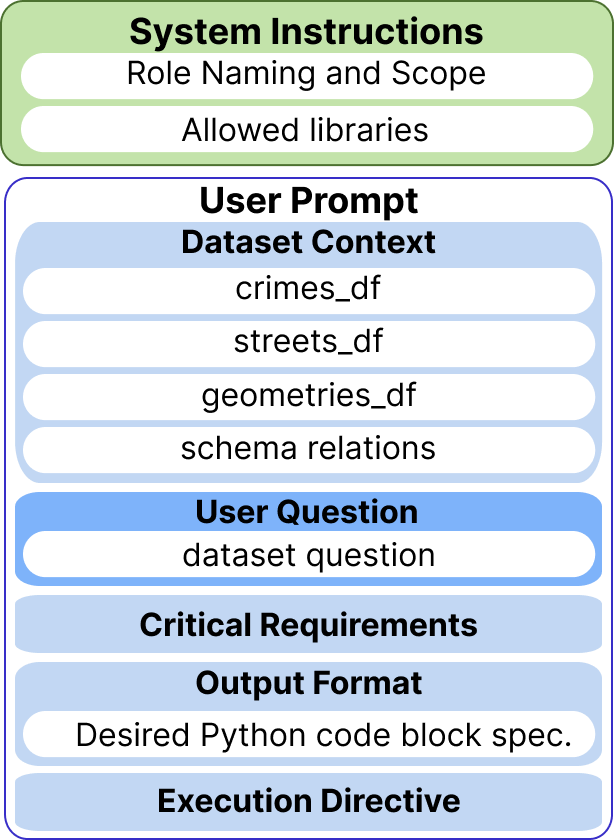
\includegraphics[width=0.29\textwidth]{images/prompt.png}
  \caption{Prompt Structure}
  \label{fig:prompt_structure}
\end{figure}


\section{Model Fine-Tuning}


% TODO: model selection
% TODO: hyperparameters and quantization
We fine-tuned the Llama-3.1-8B Instruct model \citep{Grattafiori2024Llama3, Unsloth2024WhatModel} by implementing the techniques described in \cite{Pareja2024RecipesSFT}. For the fine-tuning process, we utilized Hugging Face Transformers alongside the Unsloth library to optimize computational resources and accelerate training, completing the entire procedure in approximately 3 hours using a single NVIDIA H100 GPU with 80GB memory provided by Lightning AI. This model was chosen as it represents a balance between size (8B), data science coding capabilities \citep{Lai2022DS1000}, and compatibility with Unsloth for fast and efficient fine-tuning.

\begin{table}[H]
\centering
\caption{Fine-tuning Hyperparameters for ChinaCrimeQACode}
\label{tab:hyperparameters}
\begin{tabular}{ll}
\toprule
\textbf{Hyperparameter} & \textbf{Value} \\
\midrule
LoRA rank ($r$) & 64 \\
LoRA alpha & 16 \\
LoRA dropout & 0.0 \\
Batch size (per device) & 32 \\
Gradient accumulation steps & 4 \\
Max sequence length & 3,200 tokens \\
Training epochs & 7 \\
Learning rate & 7e-5 \\
Optimizer & \texttt{adamw\_torch\_fused} \\
Scheduler & \texttt{linear} \\
Warmup ratio & 0.1 \\
Weight decay & 0.01 \\
Quantization & 4-bit (NF4, double quant) \\
\bottomrule
\end{tabular}
\end{table}

\section{Model Evaluation}

% We adopted the approach proposed by \citep{Fleureau2024NuminaMath}, Self-Consistency Tool-Integrated Reasoning (SC-TIR) to evaluate our fine tuned model
For model evaluation, we adopted a comprehensive approach combining both automated and LLM-based assessment methods. Specifically, we used pass@k \citep{Levi2024SimpleModelInferenceScalingLaws} (with $k=16$ and multinomial sampling), where correctness was determined using an LLM-as-a-judge \citep{Li2025LLMJudge} (Appendix~\ref{appendix:prompts}) using GPT-4.1, and CodeBLEU \citep{Ren2020CodeBLEU}, which provides a purely quantitative measure of code generation quality. Additionally, we calculated the error percentage across all generated code samples to assess overall robustness. Finally, we performed Tool Integrated Reasoning (TIR) \citep{Fleureau2024NuminaMath} evaluations, allowing a single retry per question to mitigate frequent inference errors such as ZeroDivisionError and IndexError, while maintaining evaluation efficiency.

% TODO: poner que metodo de inferencia estamos usando, puede que sea greedy decoding

% The model was trained using QLoRA \citep{Dettmers2023QLoRA} with a rank of 64, alpha of 16, and a dropout rate of 0.05. 

% We employed a learning rate of 2e-4 with the AdamW optimizer and cosine learning rate scheduler with 100 warm-up steps. Training was performed for 3 epochs with a batch size of 16, using a maximum sequence length of 2048 tokens. To maintain training stability, we applied gradient clipping with a maximum norm of 1.0.

% For instruction tuning, we formatted our question-code pairs using a standard template that clearly specified the task context and expectations. Each question was prefaced with a system prompt indicating that the model should generate executable Python code to analyze crime data and answer the given question. 


\section{Case Study Inference Workflow}

% TODO: diagrama de flujo de la inferencia para estudios de caso

\section{Resume}

This section provides a detailed overview of the methodology ...

The section continues by detailing ...
